\documentclass[tikz,border=8pt]{standalone}
\usepackage{tikz}
\usepackage{tkz-euclide}
\usepackage{amsmath, amssymb}

\usetikzlibrary{angles, quotes}

\begin{document}

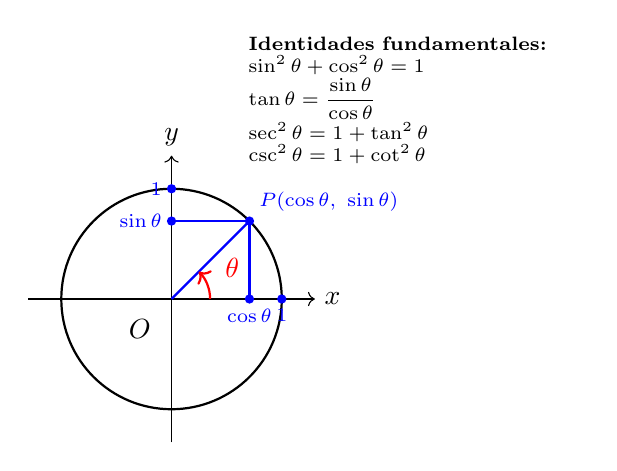
\begin{tikzpicture}[scale=1.4]

  % Circunferencia unitaria
  \draw[thick] (0,0) circle (1);
  \draw[->] (-1.3,0) -- (1.3,0) node[right] {$x$};
  \draw[->] (0,-1.3) -- (0,1.3) node[above] {$y$};
  \node[below left] at (-0.1,-0.1) {$O$};

  % Ángulo θ en primer cuadrante
  \coordinate (P) at ({cos(45)},{sin(45)});
  \draw[thick, blue] (0,0) -- (P);
  \draw[thick, blue] (P) -- (P |- 0,0);
  \draw[thick, blue] (P) -- (0,0 |- P);

  % Arco del ángulo
  \draw[->, thick, red] (0.35,0) arc (0:45:0.35);
  \node[red] at (0.55,0.28) {$\theta$};

  % Puntos y etiquetas
  \fill[blue] (P) circle (1.2pt) node[above right] {\scriptsize $P(\cos\theta,\ \sin\theta)$};
  \fill[blue] (P |- 0,0) circle (1.2pt) node[below] {\scriptsize $\cos\theta$};
  \fill[blue] (0,0 |- P) circle (1.2pt) node[left] {\scriptsize $\sin\theta$};
  \fill[blue] (1,0) circle (1.2pt) node[below] {\scriptsize $1$};
  \fill[blue] (0,1) circle (1.2pt) node[left] {\scriptsize $1$};

  % Identidades trigonométricas (compendio)
  \node[align=left, text width=4.2cm, font=\scriptsize] at (2.2, 1.8) {
    \textbf{Identidades fundamentales:}\\
    $\sin^2\theta + \cos^2\theta = 1$\\
    $\tan\theta = \dfrac{\sin\theta}{\cos\theta}$\\
    $\sec^2\theta = 1 + \tan^2\theta$\\
    $\csc^2\theta = 1 + \cot^2\theta$
  };

\end{tikzpicture}

\end{document}
